% !TEX encoding = UTF-8 Unicode

\documentclass[11pt,english]{article} % document type and language

\usepackage{babel}    % multi-language support
\usepackage{float}    % floats
\usepackage{url}      % urls
\usepackage{graphicx} % figures

\title{Float 4900497: Dissolved Oxygen DMQC}
\author{Christopher Gordon\\Fisheries \& Oceans Canada}
\date{\today}

\begin{document}

\maketitle

\section{Introduction}

The goal of this document is to summarize the results of oxygen gain
calculations made using the newly developed python package, \verb|bgcArgoDMQC|,
as well as the previously established matlab package, \verb|SAGEO2|. In the
conclusion section I will present what I believe is the best course of action.

\section{Current Status of Data}

Oxygen data is currently all in real time files, but the data mode is set
to ``A'' as the DOXY\_ADJUSTED field is populated with values. The
adjusted data uses a gain value of 1.02 - my initial instinct is this value came
from the DOXY audit produced by Josh Plant. However, the \newline
SCIENTIFIC\_CALIB\_COMMENT states the following: 

\noindent``G determined from float measurements in air. See Johnson et al., 2015, doi:10.1175/JTECH-D-15-0101.1''

However, I don't find any usable in-air data in the trajectory file (a field
for DOXY exists, but is only fillvalues), nor does the SAGE software.

In terms of flagging, any not-good DOXY data appears to be due to propogation
of flags from the physical data: 

\begin{figure}[H]
    \centering
    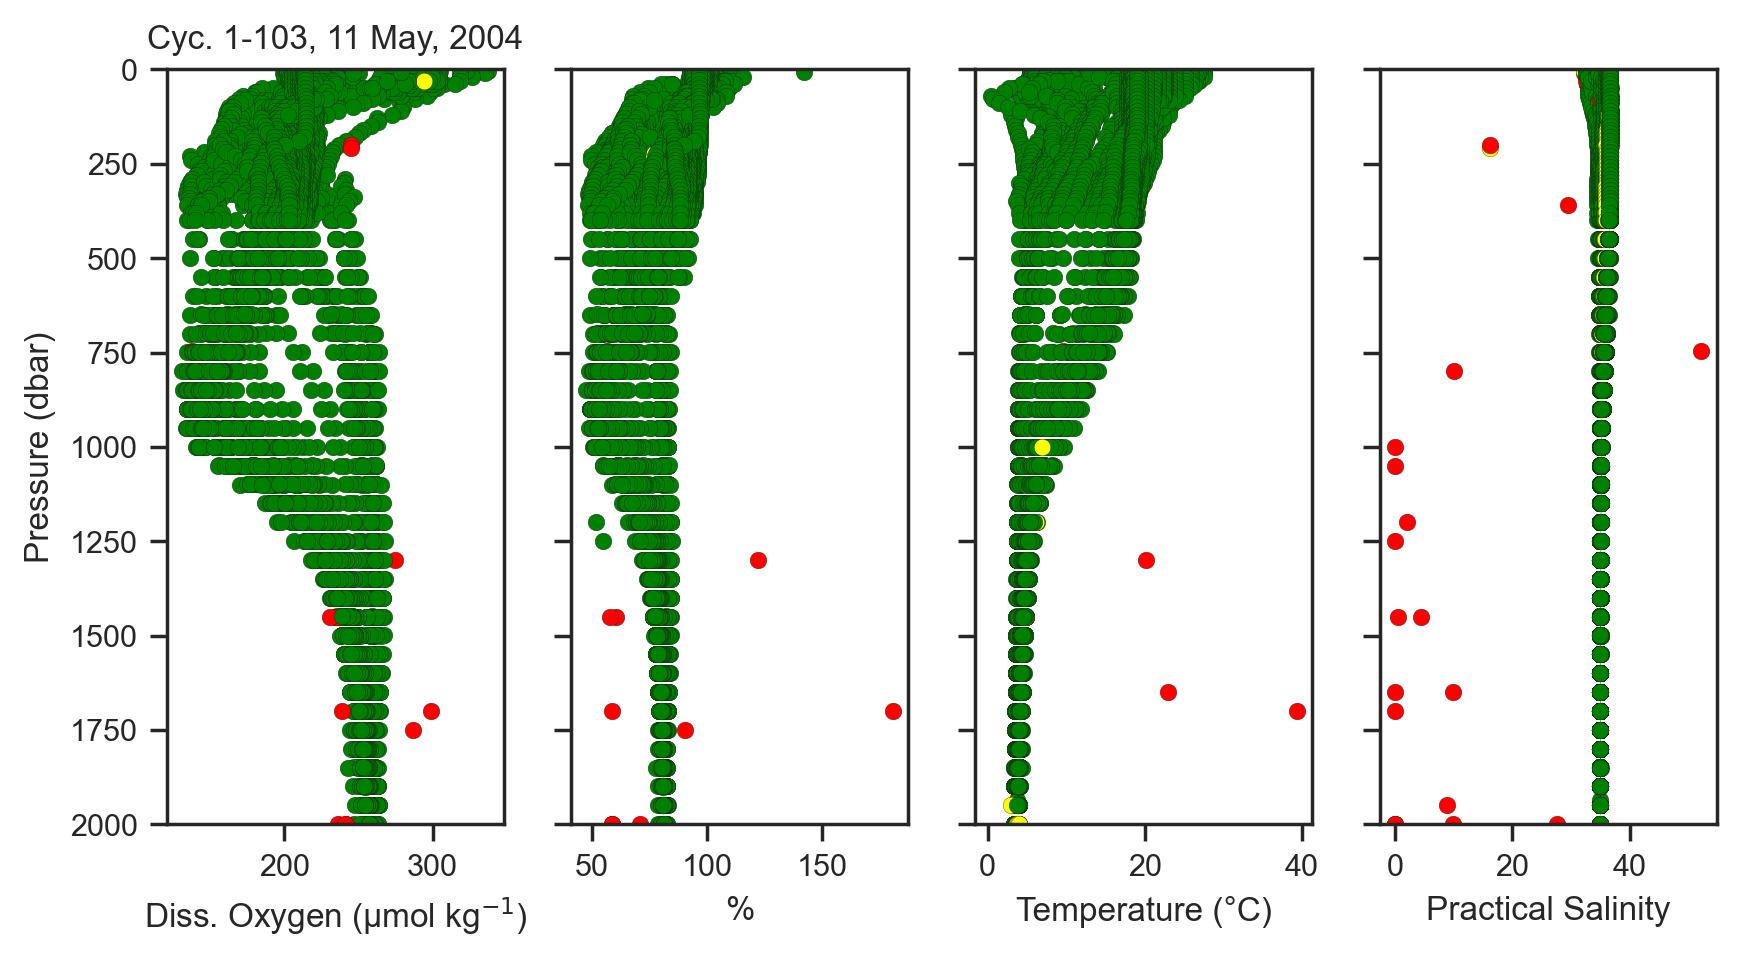
\includegraphics[width=0.8\textwidth]{../figures/4900497/qcprofiles.png}
    \caption{All float data, colour coded by quality flag}
\end{figure}

There are three points in the salinity data near the bottom of the profile that
have their QC flag set to 8 (interpolated, blue points) that look incorrect to
me. I think these values and the associated oxygen values should be set to 4.
There are 2 points in cycle 96 and 1 in cycle 100. Also - cycles 1-100 have all
gone through physical DMQC but cycles 101, 102, 103 are still in RT.

\section{Gain}

The gain calculation gives a mean gain value of 1.06.

\begin{figure}[H]
    \centering
    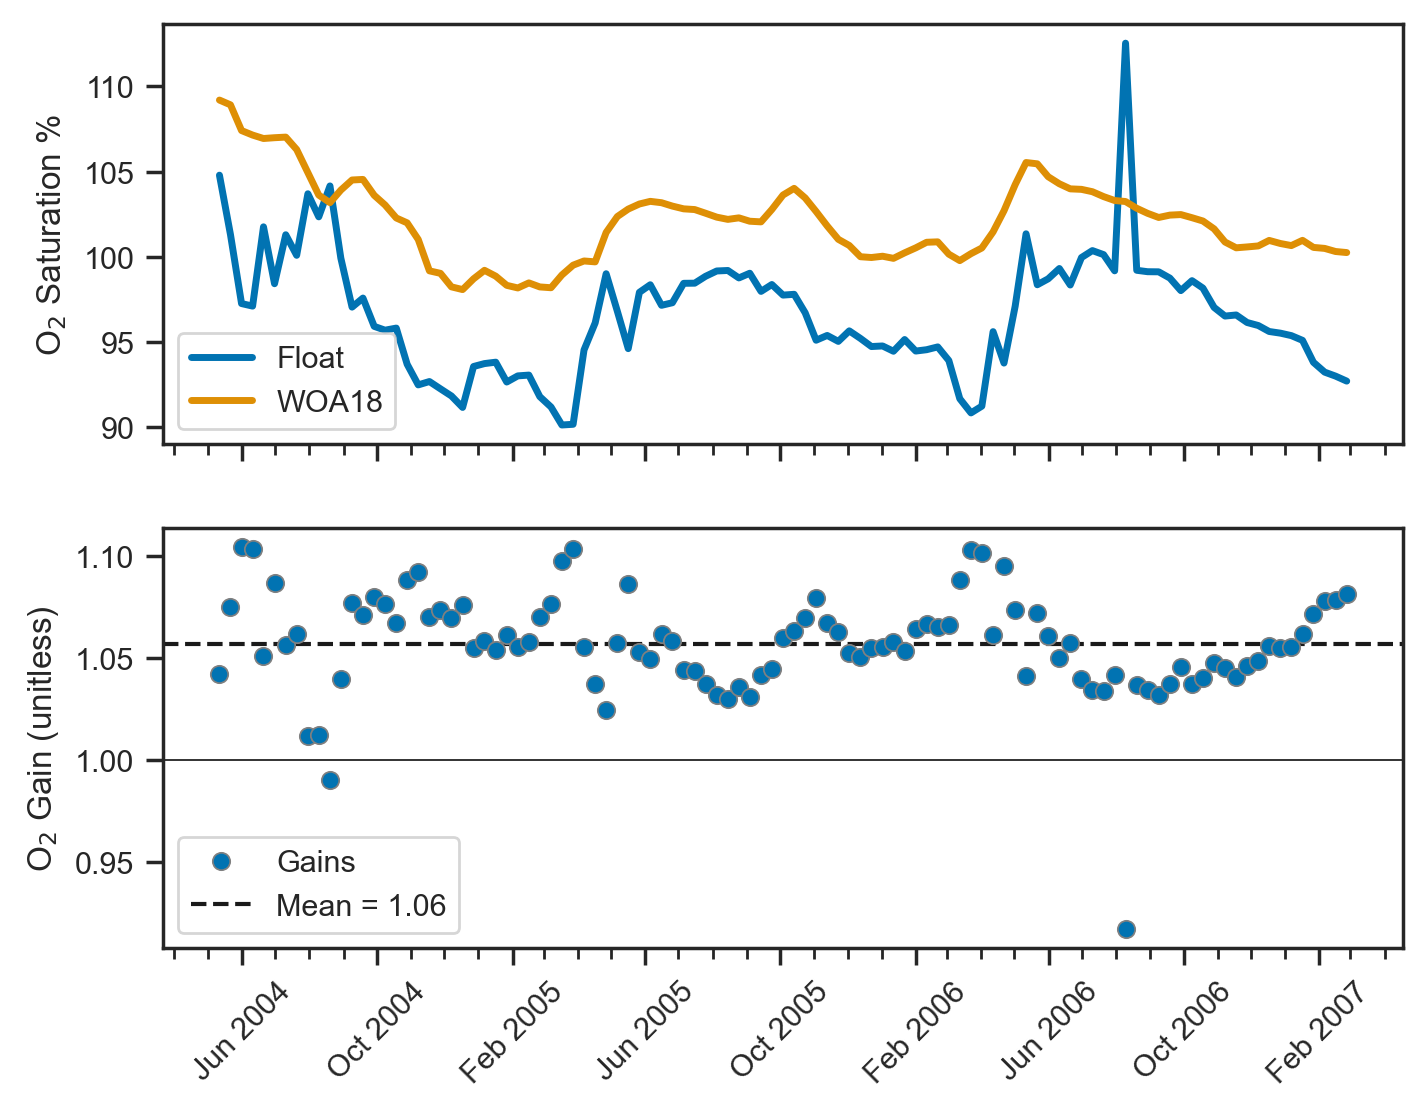
\includegraphics[width=0.8\textwidth]{../figures/4900497/gainplot.png}
    \caption{Gain plot produced by python package}
\end{figure}

The spike in August 2006 does not seem to go with the rest of the data. Upon
inspection of the individual profile, the point appears anomalous with an
oxygen saturation of 138\%.

\begin{figure}[H]
    \centering
    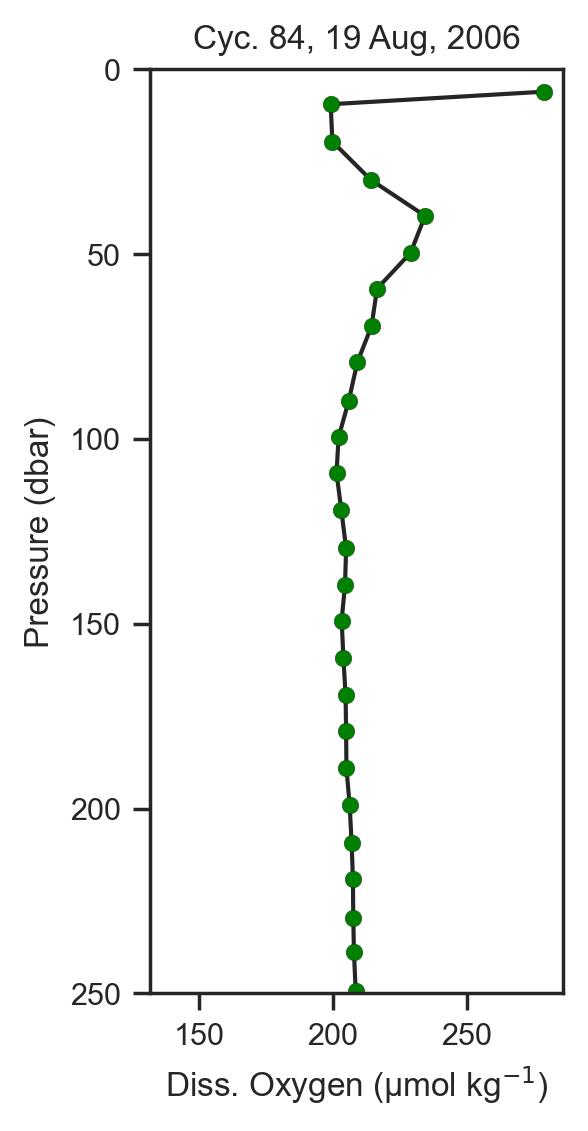
\includegraphics[width=0.25\textwidth]{../figures/4900497/anom_profile.png}
    \caption{Upper ocean data for cycle 84}
\end{figure}

I believe the top point should have its QC flag set to 4. Removing this point
however does not change the mean gain value.

\begin{figure}[H]
    \centering
    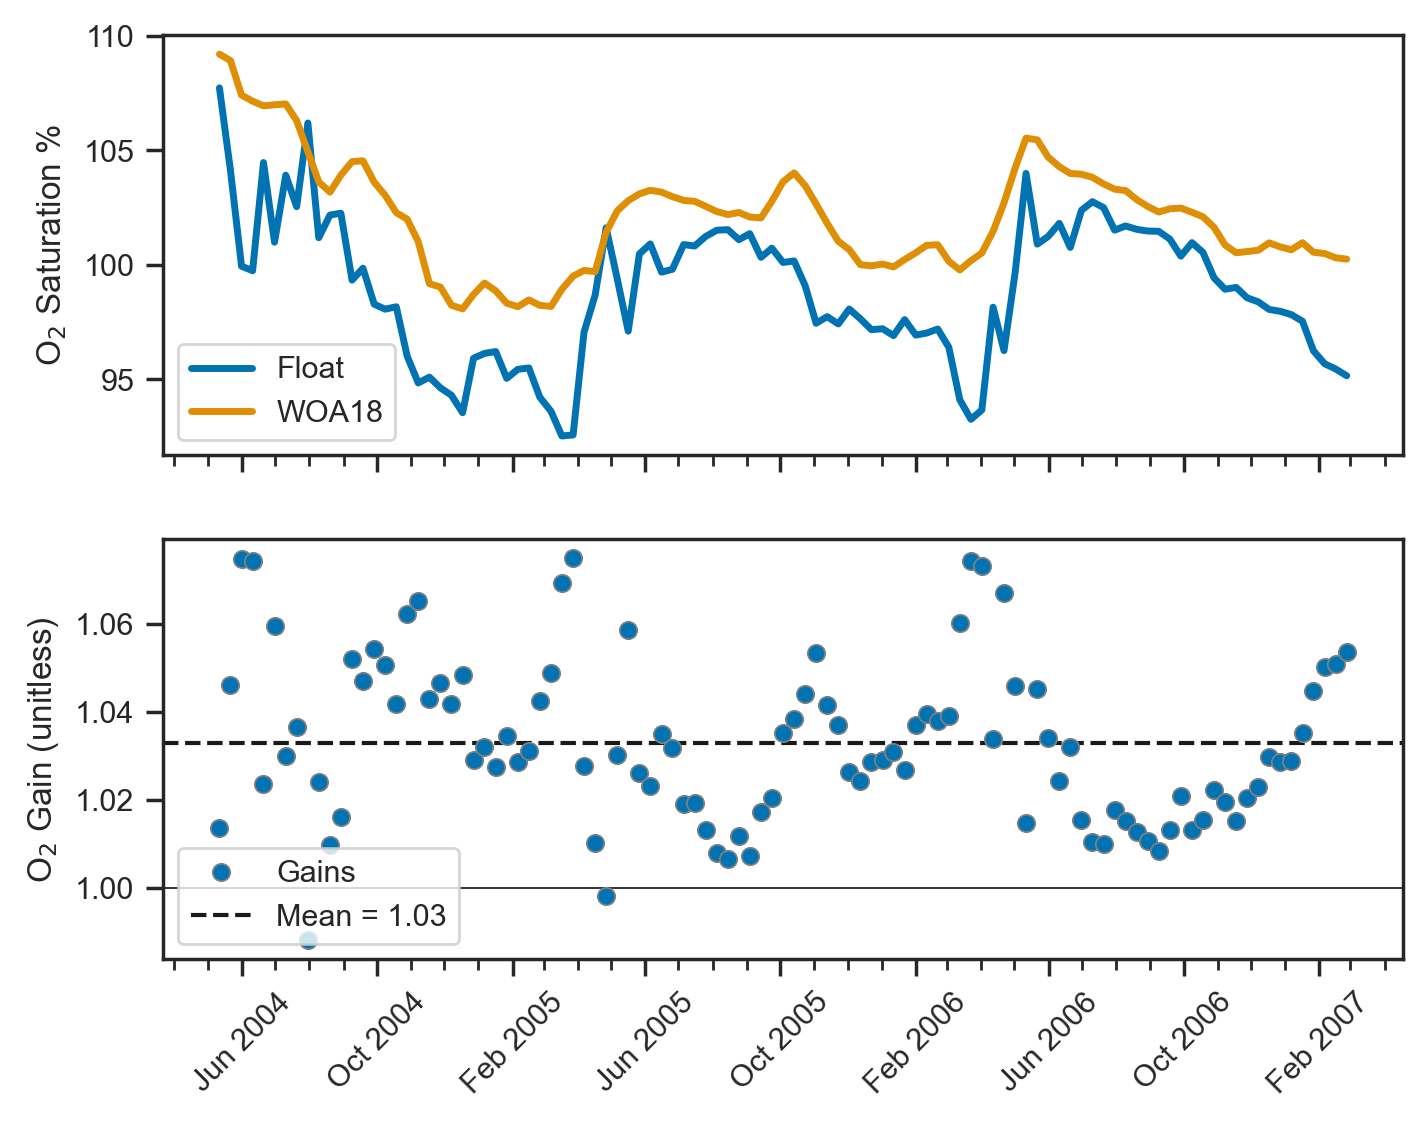
\includegraphics[width=0.8\textwidth]{../figures/4900497/new_gainplot.png}
    \caption{Gain plot repeated with anomalous point removed}
\end{figure}

Comparing the output of the python package to SAGE shows a very similar plot,
but the mean gain value is SAGE is 1.03.

\begin{figure}[H]
    \centering
    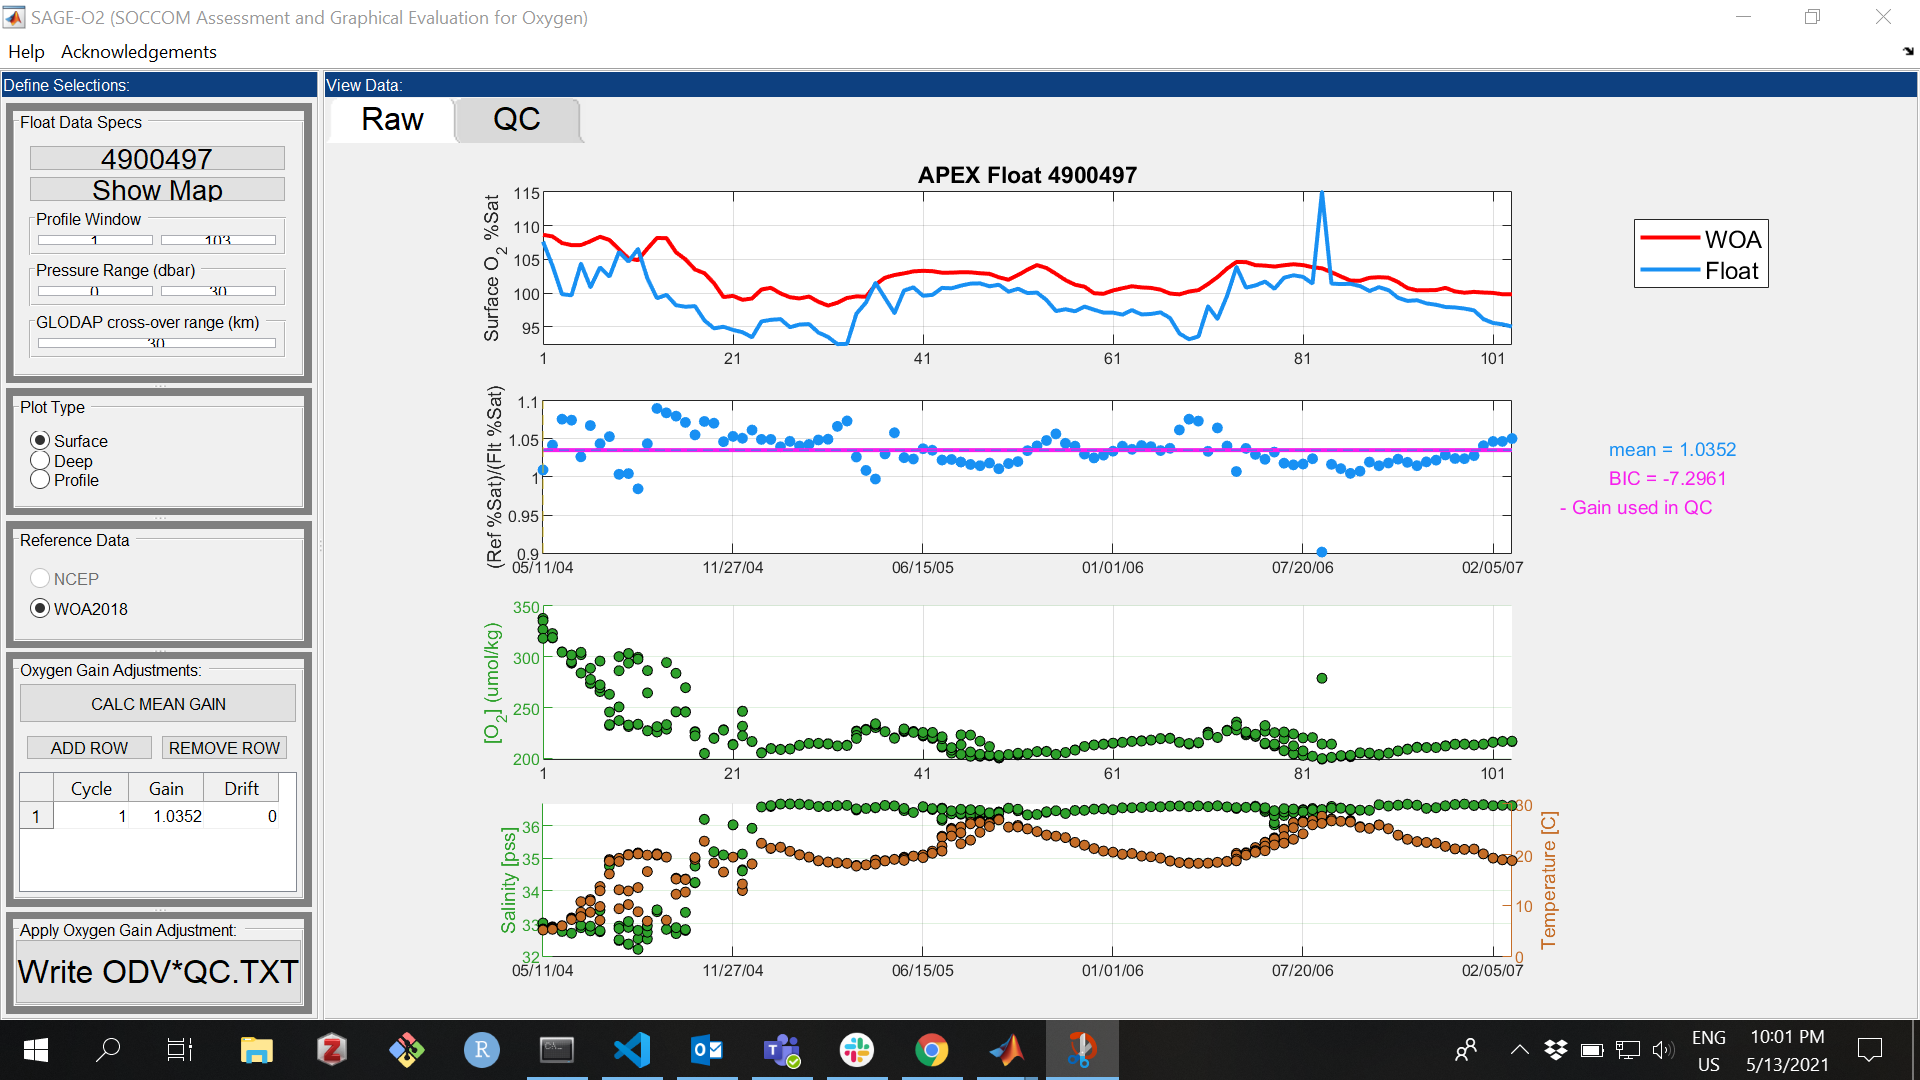
\includegraphics[width=0.8\textwidth]{../figures/4900497/SAGE_screenshot.png}
    \caption{Screenshot of SAGE software}
\end{figure}

Upon further inspection, it is clear that this is due to an underestimation of
the float oxygen saturation by the python package. The most likely reason for
this is a difference in the unit conversion from dissolved oxygen to percent
saturation. There are slightly different coefficients used depending on the model
of oxygen sensor. For now, the python package assumes an Aanderaa 4330, however
where this is an older float, it has a 3830 on it. When I tried to re-calculate
the saturation with the proper coefficients this exposed a bug in my code that
I will need to fix.

\begin{figure}[H]
    \centering
    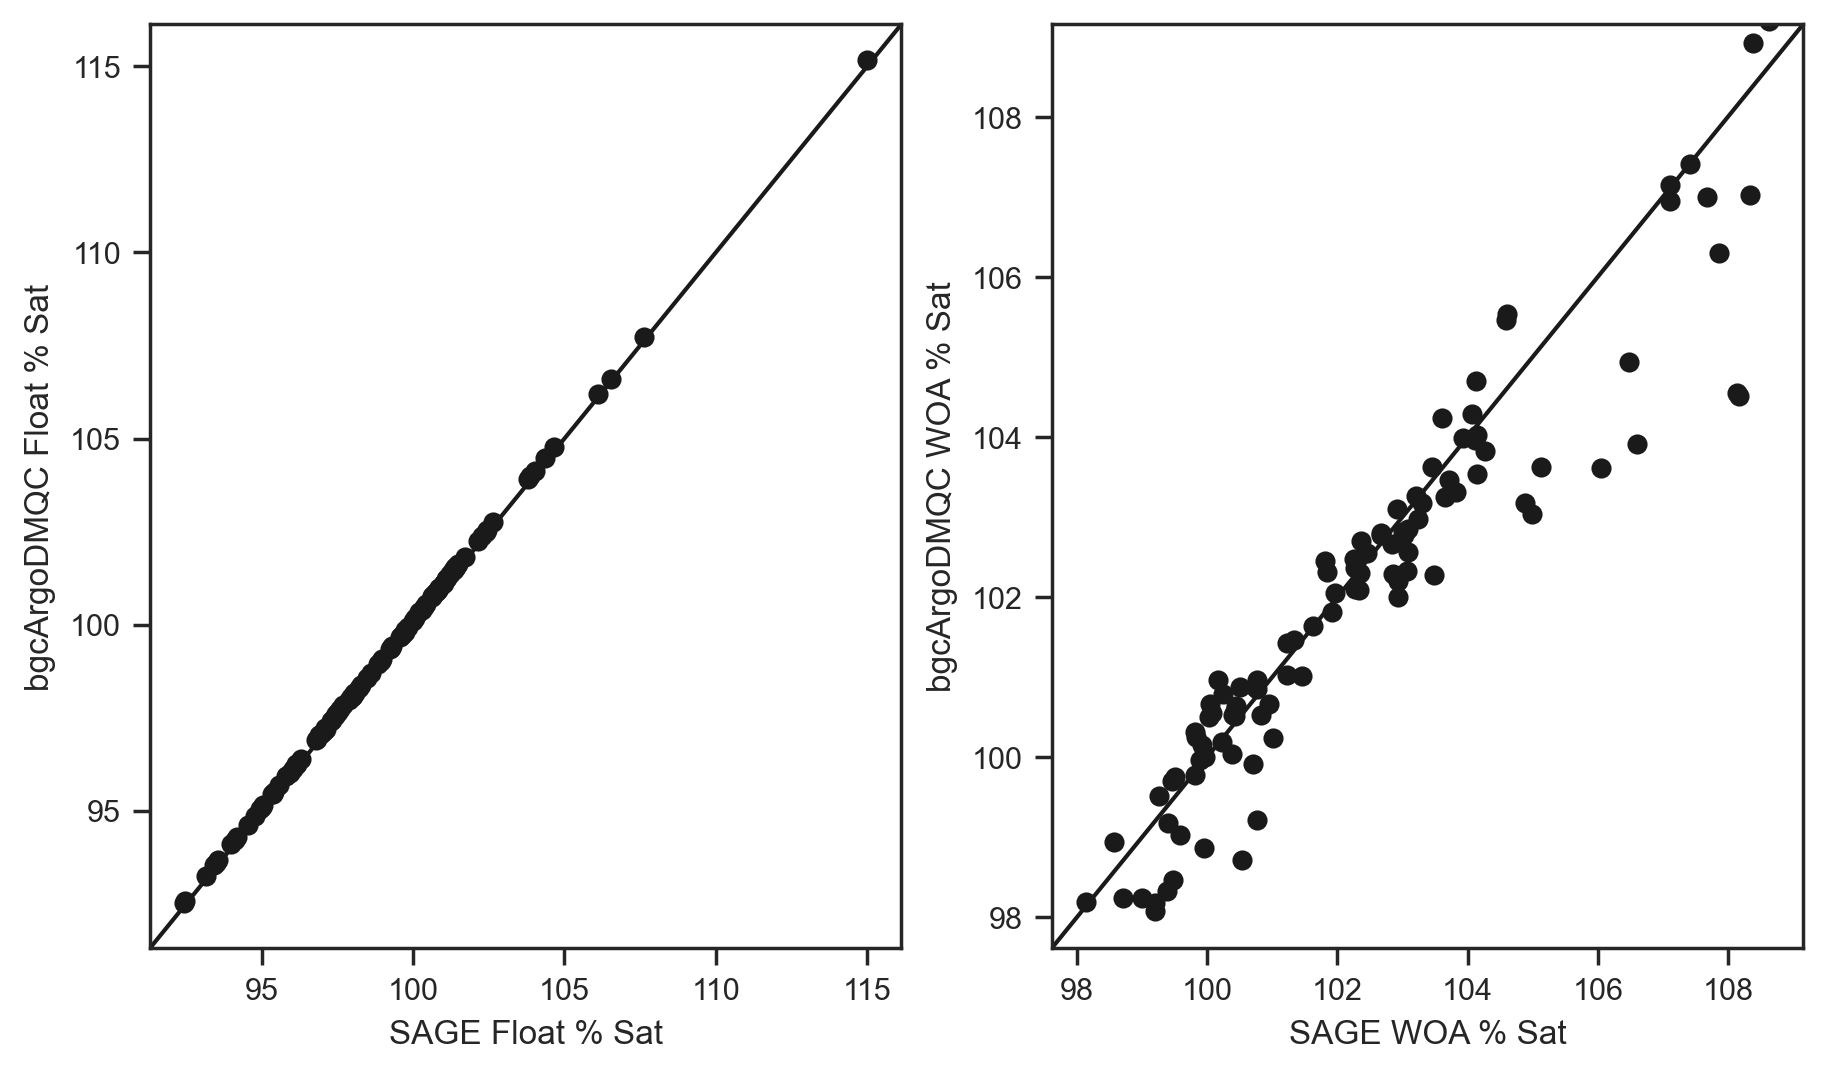
\includegraphics[width=0.8\textwidth]{../figures/4900497/sage_comparison.png}
    \caption{Comparison between matlab SAGE and python package.}
\end{figure}

There is also some differences in the interpolation of the WOA data, but these
data surround the 1:1 line and so I believe this difference is a lower
priority. Based on that I believe the SAGE code to calculate percent saturation
is more correct than mine, adjusting the float data in python gives a final mean
gain of 1.0333. 

\section{Conclusion}

In conclusion I propose the following action items:

\begin{enumerate}
    \item Change the two interpolated PSAL points from flag 8 to flag 4,
    change corresponding oxygen flags to 4 as well.
    \item Set flag for the most shallow point in cycle 84 to 4.
    \item Fill adjusted DOXY field with gain of 1.03, add appropriate comment
    SCIENTIFIC\_CALIB\_COMMENT, iterate dimension N\_HISTORY
\end{enumerate}

A final action item for the python package is to debug and fix the calcualtion
of oxygen solubility for Aanderaa 3830 optodes, and to have the package
automatically check the sensor model to do the appropriate calculation. There
is currently an open issue on the package's github page for this change.

\end{document}